%==============================================================================
% SIMTiX v2 --- IEEE Transactions on VLSI Systems manuscript (journal format).
% Build:  pdflatex simtix_tvlsi && pdflatex simtix_tvlsi
% Figures: docs/plot_vortex.py, docs/plot_lanes.py (into docs/figs/).
% \tbd{...} marks numbers still to be measured (lane builds, board run).
%==============================================================================
\documentclass[journal]{IEEEtran}

\usepackage{cite}
\usepackage{amsmath,amssymb}
\usepackage{graphicx}
\usepackage{booktabs}
\usepackage{multirow}
\usepackage{xcolor}
\usepackage{tikz}
\usetikzlibrary{positioning,fit,backgrounds,arrows.meta,calc}
\usepackage{url}
\usepackage[hidelinks]{hyperref}

\graphicspath{{../figs/}}
\setlength{\tabcolsep}{3.5pt}
\renewcommand{\arraystretch}{1.08}
\newcommand{\Fmax}{$F_{\max}$}
\newcommand{\tbd}[1]{\textcolor{red}{[#1]}}

\begin{document}

\title{SIMTiX: A Compact RISC-V SIMT Accelerator With Line-Aggregated Atomic
Operations for FPGA Systems-on-Chip}

\author{Krishna~Gorai and Bikram~Paul%
\thanks{K. Gorai and B. Paul are with the School of Computing and Electrical
Engineering, Indian Institute of Technology Mandi, Mandi 175075, India (e-mail:
kg05112001@gmail.com; bikram@iitmandi.ac.in).}}

\markboth{IEEE Transactions on Very Large Scale Integration (VLSI) Systems}%
{Gorai and Paul: SIMTiX: A Compact RISC-V SIMT Accelerator}

\maketitle

\begin{abstract}
This paper introduces SIMTiX, a RISC-V single-instruction multiple-thread (SIMT)
accelerator for FPGA systems-on-chip. Open soft GPUs either omit the memory
system that applications need or are large, and they are rarely compared on the
same device. SIMTiX has eight lanes and four warps, FP32/FP16 arithmetic, warp
shuffles, block barriers, RV32A atomic memory operations (AMOs), and a
non-blocking 16~KB L1 data cache that reaches the DDR4 of a Zynq UltraScale+
processing system. We propose line-aggregated AMOs: the memory engine serves all
lanes of an AMO that fall in one cache line with one read and one write, and
returns to every lane the value of serial execution in lane order. This reduces
the memory requests of a histogram from 2,176 to 640 and its run time by
$1.7\times$, and speeds up k-means by $1.29\times$, for 2,551 lookup tables
(LUTs). The complete board design closes timing at 101.0~MHz. We built Vortex
with four warps of eight threads for the same device with the same Vivado flow:
SIMTiX runs seven applications in $2.01\times$ less time (geometric mean) with
$4.3\times$ less estimated energy, 5\% more LUTs and 59\% fewer flip-flops.
Vortex needs 16 warps and 30\% more LUTs to come within $1.20\times$ of SIMTiX's
run time, and is then faster on GEMM and SpMV. A sweep from four to 16 lanes
shows that the memory engine, not the lanes, limits wider warps. \tbd{one
sentence with the board result}.
\end{abstract}

\begin{IEEEkeywords}
Atomic memory operations, FPGA, general-purpose GPU (GPGPU), RISC-V,
single-instruction multiple-thread (SIMT), soft processor.
\end{IEEEkeywords}

%==============================================================================
\section{Introduction}
%==============================================================================
\IEEEPARstart{F}{ield}-programmable gate array (FPGA) systems-on-chip such as the
AMD Zynq UltraScale+ combine hard processor cores with programmable logic.
Typically the processors run the control code and the logic holds fixed-function
accelerators, each synthesized for one kernel. A programmable data-parallel
engine in the logic can instead serve many kernels without a new bitstream.
Graphics processing units (GPUs) provide such an engine through the
single-instruction multiple-thread (SIMT) model: scalar threads are grouped into
warps that execute one instruction stream on a vector of lanes, and the hardware
switches between warps to hide memory latency~\cite{tesla,aamodt}.

A number of soft GPUs have been published (Section~\ref{sec:related}). The
compact ones have no cache; eGPU~\cite{egpu}, for example, reaches global data
through its shared memory. The ones with a complete memory system, such as
Vortex~\cite{vortex} and Ventus~\cite{ventus25}, are large: one Ventus streaming
multiprocessor occupies 329k LUTs. The designs are also evaluated on different
devices, with different tools and benchmarks, so their costs cannot be compared
directly.

Atomic memory operations (AMOs) are a particular problem for a soft SIMT engine.
One AMO instruction of a warp of $L$ lanes is $L$ read-modify-write operations,
and in histogram, clustering and graph kernels many of them fall in the same
cache line or on the same word. A GPU executes them in atomic units at its L2
cache~\cite{fermi}. In an FPGA system-on-chip the accelerator reaches memory
through the AXI4 ports of the processing system, which have no atomic
transactions, so the accelerator must perform every AMO itself as a read and a
write. Performed one lane at a time, the atomics become the bottleneck of these
kernels.

SIMTiX is designed from the outset as a peripheral of the processing system: the
Cortex-A53 is the host, kernel data lives in DDR4, and the complete board design,
not only the accelerator, has to close timing. SIMTiX makes the following
contributions:
\begin{enumerate}
\item \emph{Memory system}: a non-blocking L1 data cache, a memory engine with one
context per warp and an AXI4 master into DDR4, with warp shuffles, block barriers
and RV32A AMOs, in 81k LUTs of a board design that closes at 101.0~MHz
(Sections~\ref{sec:arch} and~\ref{sec:impl}).
\item \emph{Line-aggregated AMOs}: all lanes of an AMO that fall in one line are
served with one read and one masked write, and every lane receives the value of
serial execution in lane order. We give a one-lane-per-cycle and a parallel
variant, with their cost and benefit (Sections~\ref{sec:amo}
and~\ref{sec:evalamo}).
\item \emph{Same-device comparison}: Vortex~3.0 and SIMTiX are built for the same
device with the same Vivado flow and run the same seven applications, at 4, 8
and 16 Vortex warps, which separates instruction count, instructions per cycle
(IPC), area, frequency and power (Section~\ref{sec:evalvortex}).
\item \emph{Scalability}: a sweep from four to 16 lanes, which shows that the
memory engine limits wider warps and exposed a bound on the depth of the
reconvergence stack, and measurements on the board against the Cortex-A53
(Sections~\ref{sec:evallanes} and~\ref{sec:evalboard}).
\end{enumerate}
Our goal is not to compete with hard GPUs or with multi-core soft GPGPUs, but to
provide a compact programmable engine with a complete memory system beside the
host processor of a mid-size FPGA system-on-chip. The register-transfer-level
(RTL) source, kernels, testbenches, Vortex port and scripts are available at
\url{https://github.com/Krishna-Gorai/simtix}.

%==============================================================================
\section{Comparison to Other Soft GPU Architectures}\label{sec:related}
%==============================================================================
FlexGrip~\cite{flexgrip} executes CUDA binaries on an FPGA, and
FGPU~\cite{fgpu} is an OpenCL-programmed SIMT processor. MIAOW~\cite{miaow}
implements the AMD Southern Islands compute unit in RTL but models its memory
hierarchy in software. Nyami~\cite{nyuzi} is a synthesizable GPU model, and
Simty~\cite{simty} executes the RISC-V instruction set with a generalized SIMT
front end. eGPU~\cite{egpu} places 16 scalar processors and 512 threads in 5,600
Agilex logic modules and closes above 770~MHz. Vortex~\cite{vortex} extends
RISC-V with instructions for warp control, divergence and barriers, and provides
a configurable multi-core GPGPU with L1 and L2 caches, local memory and an OpenCL
stack. Ventus~\cite{ventus25} builds a GPGPU on the RISC-V vector extension; its
vector register file is 54\% of the area of a streaming multiprocessor.

\begin{table}[t]
\caption{Resource Comparison}
\label{tab:soa}
\centering\footnotesize
\setlength{\tabcolsep}{2.4pt}
\begin{tabular}{lllrrr}
\toprule
Architecture & Device & Configuration & LUTs & DSP & \Fmax\\
\midrule
FGPU~\cite{fgpu}$^a$         & Xilinx 28~nm & 2 CU $\times$ 8 PE & 57k & 48 & 250\\
FlexGrip~\cite{flexgrip}$^a$ & Xilinx 40~nm & 1 SM $\times$ 16 PE & 100k & 300 & 100\\
eGPU~\cite{egpu}             & Agilex & 1 SM $\times$ 16 SP & 5.6k$^b$ & 24 & 771\\
Ventus~\cite{ventus25}       & VU37P & 1 SM & 329k & --- & ---\\
Vortex~\cite{vortex}$^c$     & XCZU7EV & 4 warps $\times$ 8 & 80.1k & 48 & 140.8\\
SIMTiX$^c$                   & XCZU7EV & 4 warps $\times$ 8 & 84.4k & 72 & 101.6\\
\bottomrule
\end{tabular}

\vspace{2pt}
\begin{minipage}{\columnwidth}\footnotesize
$^a$As reported in~\cite{egpu}. $^b$Adaptive logic modules. $^c$Built in this
work with the same flow (Section~\ref{sec:method}). CU: compute unit; PE:
processing element; SM: streaming multiprocessor; SP: scalar processor. \Fmax\
in MHz.
\end{minipage}
\end{table}

Table~\ref{tab:soa} compares the resources of these designs, counted in lookup
tables (LUTs) and digital signal processing (DSP) blocks. This comparison is only
representative: the devices, tools and configurations differ, and the
frequencies of the earlier designs are taken from their papers. One Ventus
streaming multiprocessor needs more LUTs than the 230,400 of our device, so it
cannot be built for it. SIMTiX is closest to Vortex: both execute one scalar
RISC-V thread per lane with a few custom instructions, and Vortex can be
configured with the same warp and lane counts. We therefore built Vortex~3.0 for
our device with our flow and compare the two directly in
Section~\ref{sec:evalvortex}.

GPUs execute global atomics in atomic units at the L2 cache~\cite{fermi}, and in
the GPU model of~\cite{dab} the atomics of a warp that fall in one cache sector
form one transaction. Franey and Lipasti studied hardware support for GPU
atomics~\cite{franey}. PHI buffers and coalesces commutative updates in the
caches of a multicore~\cite{phi}, and DAB buffers GPU atomics to make them
deterministic~\cite{dab}. In software, warp-aggregated atomics combine the
same-address increments of a warp with shuffles and let one elected lane perform
a single atomic~\cite{warpagg}; this needs a commutative operation on one address
and a change to the kernel. Vortex~3.0 sends the AMO of each lane as a separate
request to a bank of its last-level cache, which reads, modifies and writes one
word per request. SIMTiX aggregates in the memory engine of the core, ahead of the
L1. The aggregation covers lanes on different words of one line and lanes on the
same word, applies to every RV32A AMO including swap, minimum and maximum, returns
the old value of every lane, and needs no change to the kernel.

%==============================================================================
\section{Architecture}\label{sec:arch}
%==============================================================================
\begin{figure*}[t]
\centering
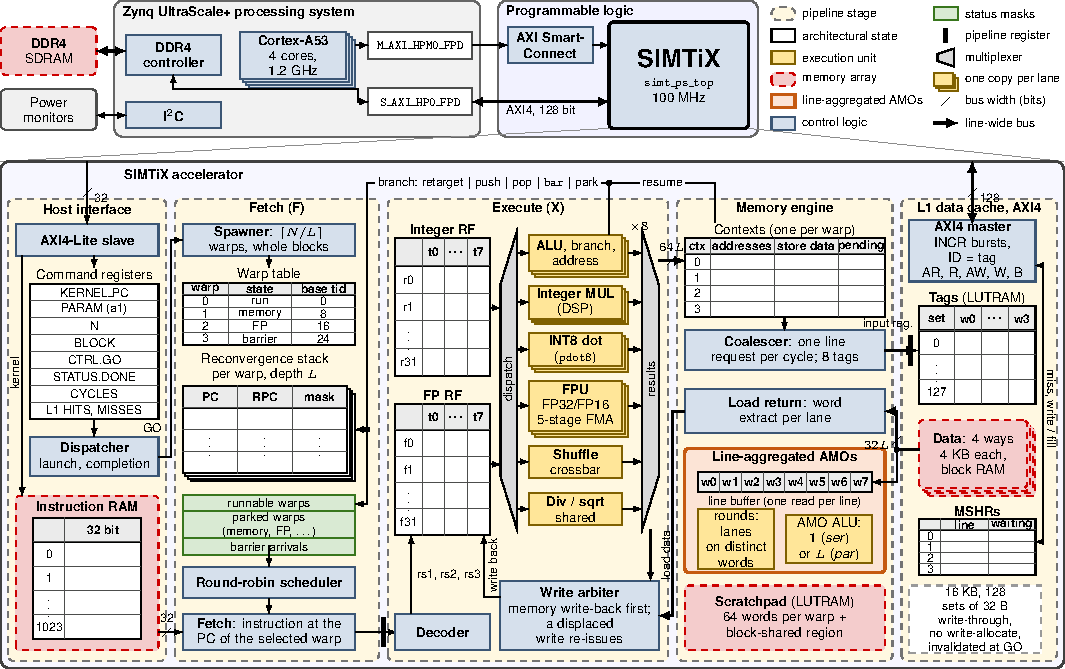
\includegraphics[width=\textwidth]{simtix_arch_v3.pdf}
\caption{SIMTiX on the ZCU104 (top) and the accelerator by pipeline stage
(bottom). The Cortex-A53 writes the kernel and the launch parameters over
AXI4-Lite and polls for completion. The scheduler selects a runnable warp, whose
instruction is fetched (F) at the top of its reconvergence stack, decoded and
executed (X) on the eight lanes, or parks the warp on a multi-cycle unit; branch
outcomes and barriers update the stack and the status masks. A memory
instruction passes to the context of its warp, which coalesces it into line
requests and executes AMOs one line at a time, and resumes the warp when its last
response returns. Line requests reach DDR4 through the L1 data cache, the AXI4
master and the port S\_AXI\_HP0. The register files, the L1 tags and the
scratchpad are in LUTRAM. RF: register file; tid: thread ID; RPC: reconvergence
PC.}
\label{fig:arch}
\end{figure*}

SIMTiX is organized in a typical SIMT machine topology, but is designed from the
start as a peripheral of an FPGA system-on-chip. A kernel is launched for $N$
threads. We will use the term \emph{warp} to denote $L$ threads that execute one
instruction together, one per \emph{lane}, and \emph{block} to denote a group of
$2^b$ warps that can synchronize at a barrier and share a scratchpad. $W$ warps are
resident at a time; the board design has $W=4$ and $L=8$. Fig.~\ref{fig:arch}
shows the board system (top) and the accelerator grouped by pipeline stage
(bottom).

\subsection{System and Host Interface}
One Cortex-A53 core runs a bare-metal host program. It reaches the accelerator
through the PS master port M\_AXI\_HPM0\_FPD and an AXI SmartConnect, which
converts the transactions to AXI4-Lite. The \emph{AXI4-Lite slave} of the
accelerator decodes two windows. The first holds the \emph{command registers}:
the kernel PC, the address of the kernel's parameter block, the thread count $N$,
the block size and GO, and, for reading, DONE, the cycle count of the last
launch, the L1 read hits and misses, and a sticky AXI error flag. The second is
the \emph{instruction RAM}, 1,024 32-bit words, into which the host writes the
kernel. When the host writes GO, the \emph{dispatcher} invalidates the L1, starts
the warps, counts cycles until the last warp finishes, and sets DONE.

Kernel data lives in DDR4, which the accelerator reaches through its AXI4 master
and the 128-bit high-performance port S\_AXI\_HP0 of the processing system (PS).
This port is not coherent with the A53 caches, so the host cleans its data cache
before GO and invalidates it after DONE. The I$^2$C controller of the PS reads the
board's power monitors (Section~\ref{sec:evalboard}).

\subsection{Fetch Stage}
The \emph{spawner} divides the threads into $\lceil N/L\rceil$ warps and places
one per cycle into a free slot of the \emph{warp table}, so a slot is refilled as
soon as its warp finishes; the last warp is masked if $N$ is not a multiple of
$L$. A block is spawned whole into a group of $2^b$ slots, so its warps are always
resident together. The warp table holds the state of each slot and the thread ID
of its lane~0. A warp is running, finished, at a barrier, or parked on a
multi-cycle unit.

Each warp has a \emph{reconvergence stack}~\cite{fung,aamodt} whose frames hold a
PC, a reconvergence PC (RPC) and an active mask; the top frame gives the warp's PC
and the lanes that execute. A uniform branch only changes the PC of the top frame.
When the lanes of a warp disagree, the branch diverges: a forward branch pushes
the not-taken lanes with the branch target as RPC, and a backward branch (a loop)
pushes the lanes that stay in the loop with the fall-through PC as RPC. A frame
whose PC reaches its RPC is popped in an issue slot of its own, and the warp
continues with the lanes of the frame below. Every pushed frame holds a strict,
non-empty subset of the lanes of the frame below it, so a warp never needs more
than $L$ frames, and we set the depth to $L$.

The \emph{status masks}, derived from the warp table, give the runnable warps, the
parked warps and the warps at a barrier. A warp at \texttt{bar} waits until every
live warp of its block has arrived. The \emph{round-robin scheduler} selects the
next runnable warp after the one issued last, and the \emph{fetch} block reads the
instruction at the PC of its top frame into the pipeline register between the two
stages.

\subsection{Execute Stage}
The \emph{decoder} accepts RV32I, the RV32M \texttt{mul}, the RV32A AMOs without
load-reserved and store-conditional, and the single- and half-precision
floating-point instructions. Three custom instructions use the \emph{custom-0}
opcode space: \texttt{pdot8}, a dot product of four signed or unsigned 8-bit
integer (INT8) pairs; \texttt{shfl.\{idx,up,down,xor\}}; and \texttt{bar}.

The integer \emph{register file} (RF) has two read ports and the floating-point RF
three, for the fused multiply-add (FMA). Both hold 32 registers per thread in
distributed RAM (LUTRAM), one bank per lane addressed by warp and register. We
moved the RFs from flip-flops to LUTRAM because a flip-flop RF needs a 128-to-1
multiplexer per lane and read port; this reduced the LUTs of the integer
accelerator from 170,868 to 30,088. A register not yet written in a launch reads
its initial value (the thread ID for \texttt{a0}, the launch arguments for
\texttt{a1}--\texttt{a4}, zero otherwise), so no cycles are spent clearing the RFs.

The \emph{dispatch} multiplexer sends the operands of the active lanes to the
selected unit. The \emph{ALU} of each lane executes the integer instructions,
evaluates branch conditions and computes memory addresses; its branch outcomes
update the reconvergence stack over the control bus at the top of
Fig.~\ref{fig:arch}. All other units take more than one cycle, and the warp parks
until its result returns while the scheduler issues other warps. Each lane has a
pipelined integer multiplier on DSP blocks, an INT8 dot-product unit, and an
FP32/FP16 unit (\emph{FPU}) for addition, multiplication, the four FMA variants,
comparisons, minimum and maximum, sign injection, conversions and
classification. The FPU has five pipeline stages, and its 48-bit significand
product is formed on a $24\times24$ cascade of DSP blocks. FP16 operations widen
their operands to FP32, use the FP32 datapath and round the result to FP16. This
double rounding is innocuous for addition, multiplication and conversions because
$24\ge2\cdot11+2$~\cite{figueroa}; the FMA is not covered by that bound, so we
round its FP32 intermediate to odd, which makes the final rounding to FP16
correct. We checked the units bit-exactly against an IEEE-754
reference~\cite{ieee754} on 116,089 arithmetic and 100,884 conversion vectors
that cover every rounding mode.

Two units are shared by the lanes. The \emph{shuffle crossbar} reads a register of
another lane, selected by an index, an offset up or down, or an XOR with the lane
number, and writes it to every active lane; shuffles implement log-step
reductions and scans within a warp. Divide and square root use one
digit-recurrence unit through which the active lanes pass in turn; a unit per
lane cost 3.7k LUTs. The \emph{result} multiplexer collects the results, and the
\emph{write arbiter} grants the single write port of each RF bank. A load
returning from the memory engine has priority. A compute result displaced by it
is not committed, and its warp issues the instruction again in the next cycle;
this is safe because the displaced instruction has written nothing.

\subsection{Memory Engine}
A load, store or AMO leaves the execute stage with the addresses and store data
of all lanes and enters the \emph{context} of its warp, which also holds the mask
of the lanes still pending. We provide four contexts, one per warp, so that a warp
waiting for memory does not block the memory accesses of the others
(Section~\ref{sec:evalmem}). Each cycle the \emph{coalescer} takes one context in
rotating order and sends one line request for its lowest pending lane together
with every pending lane whose address lies in the same line; this is
\emph{coalescing}. A store merges the bytes of these lanes into the line under
byte enables. Each request carries one of eight tags, and responses may return in
any order. The \emph{load return} block extracts the word, half-word or byte of
each lane and writes it into the RF through the write arbiter. A context finishes
when no lane is pending and every response, writes included, has returned, and it
then resumes its warp.

An AMO is a read and a write of one line, and its context holds the request port
from the read to the write so that no other request reaches the line in between.
The \emph{line-aggregated AMO} block applies all the lanes of the line to a
buffered copy (Section~\ref{sec:amo}). Two address apertures go to the
\emph{scratchpad} instead: 64 words per warp, and a region shared by the warps of
a block. The scratchpad is one single-port LUTRAM, so it serves one lane per
cycle. The RV32A AMOs (add, swap, and, or, xor, signed and unsigned minimum and
maximum) work on global and scratchpad addresses.

\subsection{L1 Data Cache and AXI4 Master}\label{sec:l1}
The L1 holds 16~KB in four ways. Its line is the memory engine's line, so at eight
lanes it has 128 sets of 32 bytes. A request first enters an \emph{input
register} with one skid entry, so the lookup starts from flip-flops
(Section~\ref{sec:closure}). The \emph{tags} are in LUTRAM and the valid bits in
flip-flops; the \emph{data} of each way is one block-RAM bank, and a hit answers
two cycles after its grant. A miss allocates one of four miss-status holding
registers (\emph{MSHRs}); a later miss to the same line joins it, and the
returning line answers all of its requests. The cache writes through without
allocating on a write miss. We chose write-through because, with GO invalidating
the L1, DDR4 then holds every result at DONE and the host needs no flush from the
accelerator. The \emph{AXI4 master} turns a line request into an incrementing
burst of $32L/128$ beats; the AXI ID is the request tag, and read beats are
collected per ID.

%==============================================================================
\section{Line-Aggregated Atomic Memory Operations}\label{sec:amo}
%==============================================================================
With one read-modify-write per lane, an AMO whose $k$ active lanes fall in one
line costs $k$ reads and $k$ writes, and behind a write-through L1 every write
also travels to DDR4. We aggregate the lanes by line instead. Let $P$ be the
pending lanes of an AMO context, $a_i$ the address of lane $i$, and $\ell=\min P$
the lead lane. The engine forms the group
$G=\{i\in P:\mathrm{line}(a_i)=\mathrm{line}(a_\ell)\}$ and
\begin{enumerate}
\item reads the line once into a line buffer;
\item applies the lanes of $G$ to the buffer in \emph{rounds}: a round applies
every remaining lane $i\in G$ for which no lower remaining lane of $G$ addresses
the same word; an applied lane receives the old word as its result and the buffer
word is replaced by the AMO's new value;
\item writes the line back with one request whose byte enables cover the words
that changed; and
\item removes $G$ from $P$ and repeats while $P$ is not empty.
\end{enumerate}
Within a round all lanes address different words and are independent; across
rounds the lanes on one word are applied in ascending lane order. The final memory
contents and every returned value are therefore those of executing the lanes one
at a time in ascending lane order, which is what the per-lane engine does. A
group needs as many rounds as the largest number of its lanes on one word.
\begin{figure*}[t]
\centering
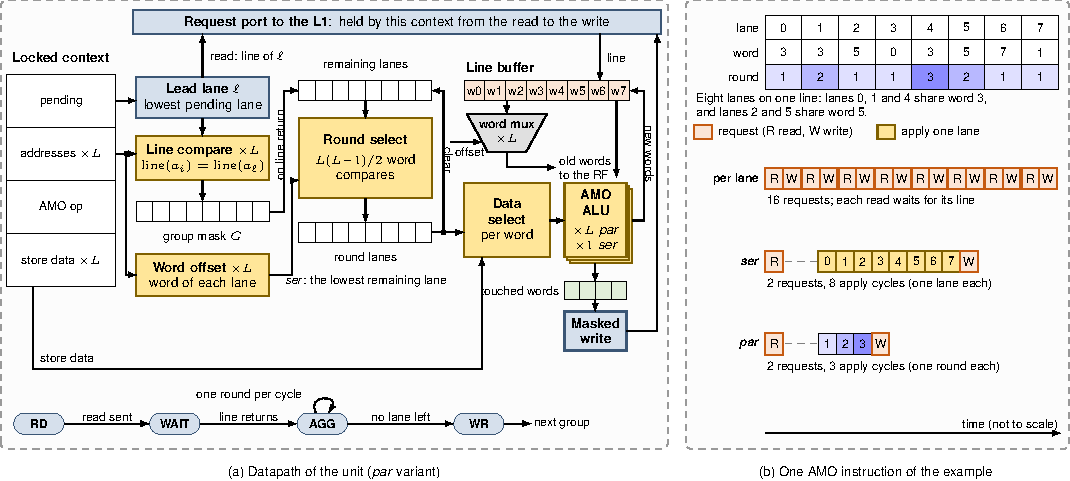
\includegraphics[width=\textwidth]{simtix_amo.pdf}
\caption{Line-aggregated AMOs. (a) Datapath of the unit in the parallel variant;
the serial variant applies the lowest remaining lane with one ALU and needs no word
compares. RD, WAIT, AGG and WR are the read, wait, apply and write states of the
context. (b) An AMO whose eight lanes address words of one line: lanes 0, 1 and 4
share word~3 and lanes 2 and 5 share word~5, so the parallel variant applies the
group in three rounds.}
\label{fig:amo}
\end{figure*}

Fig.~\ref{fig:amo}(a) shows the datapath. The lead lane and $L$ line
comparators form $G$, and the read request carries the line of $\ell$. When the
line returns, it is loaded into the line buffer and $G$ into the remaining-lanes
mask. In each cycle of the apply phase the round select picks the lanes of the
round, which takes $L(L{-}1)/2$ compares of word offsets, 28 at eight lanes. The
word multiplexers give each applied lane its old word, which returns to the RF
through the write arbiter in a cycle without a load write-back. The AMO ALUs
compute the new words, which replace their words in the buffer, and the words
written collect into the byte enables of the one masked write. A four-state
machine holds the request port from the read to the write.
Fig.~\ref{fig:amo}(b) follows one AMO instruction: per lane it needs 16 requests,
and aggregated it needs two, with eight apply cycles in the serial variant and
three in the parallel one.

We implemented both datapaths. The serial variant (\emph{ser}) has one AMO
arithmetic unit and applies the lowest remaining lane in each cycle, so the lanes
follow lane order; the parallel variant (\emph{par}) has one unit per word and
applies a whole round per cycle. Both return the same values. Out of context at 100~MHz the memory engine without
aggregation uses 10,705 LUTs, the serial variant 13,256 (2,551 more) and the
parallel variant 16,628 (5,923 more). In the board design the parallel variant
missed 100~MHz by 0.119~ns while the serial one met it, so the serial variant is
the default and the parallel one a build parameter.

A dedicated kernel issues colliding \texttt{amoadd}, \texttt{amomax} and
\texttt{amoswap} instructions and checks every returned value and the final memory
against a serial model. It and a histogram run with and without aggregation under
seven memory configurations, from a zero-latency memory to the L1 with only two
sets, which forces evictions, and the L1 behind the AXI4 master with an
out-of-order memory model.

%==============================================================================
\section{Implementation and Timing Closure}\label{sec:impl}
%==============================================================================
SIMTiX is written in SystemVerilog. Twenty-one self-checking testbenches, in 28
configurations of memory latency, ordering and cache, run under Vivado's simulator
and under Verilator~5.020 in continuous integration. We implemented all designs
with Vivado~2025.1 for the XCZU7EV-2 device of the ZCU104 (230,400 LUTs, 460,800
flip-flops, 312 block RAMs and 1,728 DSP blocks). The board design is a block
design of the PS, an AXI SmartConnect and the accelerator, implemented in context
into the bitstream that runs on the board. Every frequency we report is that of a
routed design: with worst setup slack WNS at a 10~ns constraint,
\Fmax${}=1/(10~\mathrm{ns}-\mathrm{WNS})$. None is a median over placement runs or
an estimate before routing.

\subsection{Floating-Point Datapath}
The floating-point datapath is 2.5 times the area of the integer engine and,
placed, is limited by routing rather than by logic depth. With a two-stage FMA the
eight-lane engine closed at 78~MHz out of context, with its worst path in the
first FMA stage and 58\% of the delay in routing. Sharing one divide and
square-root unit among the lanes removed 3.7k LUTs and raised this to 84~MHz with
the FMA unchanged. A four-lane build reached only 79.7~MHz, which showed that the
limit lay inside one lane's FMA rather than in the total area. A three-stage FMA
then closed at 100.7~MHz and moved the worst path to the register-file read. In
the deployed unit the significand product is fully pipelined on DSP blocks, which
makes the unit five stages deep.

\subsection{Memory Path}\label{sec:closure}
Adding the L1 and the aggregated AMOs to the board design first missed 100~MHz by
2.478~ns with 16,301 failing endpoints. The worst path was a single-cycle loop of
30 logic levels, 76\% of it routing: from the pending-lane masks of a memory
context through port arbitration and address selection into the L1 tag compare,
the hit, the completion of the context and the warp's resume into the PC of its
reconvergence stack. Four changes closed it. The L1 registers its input. A
context completes from registered state and the cycle's responses, which is valid
for a memory that never answers in the request cycle. The L1 chooses one cycle
ahead which waiting read it answers next. A post-route physical optimization pass
was added. The input register costs 1.5--2.5\% of the total cycles of the
applications.

\begin{table}[t]
\caption{Implementation Results on the XCZU7EV-2 at a 100~MHz Constraint}
\label{tab:impl}
\centering\footnotesize
\setlength{\tabcolsep}{2.6pt}
\begin{tabular}{lrrrrrr}
\toprule
Design & LUT & FF & BRAM & DSP & \Fmax & Power\\
 & & & & & (MHz) & (W)\\
\midrule
Board design$^a$       & 81,060 & 23,910 & 16 & 72 & 101.0 & 4.19\\
SIMTiX, 8 lanes$^b$    & 84,443 & 31,959 & 16 & 72 & 101.6 & 1.10\\
SIMTiX, 4 lanes$^b$    & 43,119 & 17,555 & 8  & 36 & 113.5 & 0.94\\
SIMTiX, 16 lanes$^b$   & \tbd{} & \tbd{} & \tbd{} & \tbd{} & \tbd{} & \tbd{}\\
L1 data cache$^c$      & 2,628  & 2,369  & 16 & 0  & 162.2 & ---\\
Mem. engine, base$^c$  & 10,705 & --- & 0 & 0 & --- & ---\\
Mem. engine, \emph{ser}$^c$ & 13,256 & --- & 0 & 0 & --- & ---\\
Mem. engine, \emph{par}$^c$ & 16,628 & --- & 0 & 0 & --- & ---\\
\bottomrule
\end{tabular}

\vspace{2pt}
\begin{minipage}{\columnwidth}\footnotesize
$^a$In context with the processing system; whole-device power, of which the
processing system 2.64~W and the accelerator 0.83~W dynamic.
$^b$\texttt{simt\_ps\_top} out of context through the flow of
Section~\ref{sec:evalvortex}; vectorless power.
$^c$Out of context; base is the engine without aggregation. The engine of the
board design omits the path that answers a request in its own cycle, and its
\emph{ser} variant then uses 12,576 LUTs. BRAM counts RAMB36 tiles.
\end{minipage}
\end{table}

Table~\ref{tab:impl} lists the results. The board design closes timing at
101.0~MHz ($+0.098$~ns at 100~MHz), with the stage-0 addition of a lane FPU the
critical path. The accelerator uses 35\% of the device's LUTs and 0.83~W of
dynamic power, against 2.64~W for the PS.

%==============================================================================
\section{Evaluation}\label{sec:eval}
%==============================================================================
\subsection{Methodology}\label{sec:method}
We wrote seven applications in RISC-V assembly, with one thread per output
(Table~\ref{tab:apps}): FP32 matrix multiplication (GEMM), sparse matrix-vector
product in compressed sparse row format (SpMV), two sweeps of a five-point Jacobi
stencil, the assignment step of k-means with AMO accumulation of the cluster
sums, level-synchronous breadth-first search (BFS) with one launch per level and
an \texttt{amoor} flag, an inclusive prefix sum (scan) built from a block scan
with shuffles, block-shared memory and a barrier and a second pass that adds the
block totals, and a two-layer INT8 multilayer perceptron (MLP) with
\texttt{pdot8}, requantization and a rectified linear unit. The generator computes
FP32 references with one exact rounding per operation, and every output word is
compared bit-exactly.

For SIMTiX, the board top runs in simulation, driven over AXI4-Lite as the A53
drives it, with an AXI4 memory model of 24 cycles of latency, out-of-order
responses and random ready stalls. Cycles come from the accelerator's counter,
and instructions are the warp instructions issued.

For Vortex we used release~3.0 with one core of four warps of eight threads,
RV32IMAF with the A extension, and its defaults otherwise: 16~KB 4-way
instruction and data caches with 64-byte lines, a write-back data cache, local
memory, and the Xilinx floating-point IP cores. We ported the applications to its
\texttt{vx\_spawn2} interface with the same algorithms, one thread per output and
the same order of floating-point operations, compiled them with its LLVM at
\texttt{-O3}, and checked them against the same references. They run in Vortex's
RTL simulator with its memory behind a 128-bit bus, the width of the HP port, and
with the FMA, divide and square-root latencies of the IP cores in the netlist (16,
28 and 28 cycles). Vortex counts its retired warp instructions, including its
divergence and predicate instructions.

Both designs are implemented out of context with Vortex's own Vivado script and
strategy (performance-optimized synthesis with retiming, extra timing
optimization and aggressive physical optimization before and after routing) at a
100~MHz constraint, and their power is estimated vectorless with a toggle rate of
12.5\%. Run time is cycles divided by each design's \Fmax, and energy is the power
at 100~MHz times the cycles times 10~ns. On the board, the applications run on
DRAM-sized inputs (Section~\ref{sec:evalboard}).

\begin{table}[t]
\caption{Applications, Inputs and Results on SIMTiX (8 Lanes, Simulation)}
\label{tab:apps}
\centering\footnotesize
\setlength{\tabcolsep}{2.6pt}
\begin{tabular}{llrrrrl}
\toprule
App. & Simulated input & Cycles & IPC & Util. & L1 hit & Board input\\
\midrule
GEMM    & $32^3$               & 45,902  & 0.69 & 100\% & 93\% & $256^3$\\
SpMV    & $512^2$, $\le$16/row & 26,295  & 0.43 & 59\%  & 88\% & $65{,}536^2$\\
Stencil & $32^2$, 2 sweeps     & 17,529  & 0.48 & 100\% & 88\% & $512^2$, 4\\
k-means & 1,024, $k=8$         & 36,935  & 0.66 & 100\% & 93\% & $2^{18}$, 16\\
BFS     & 1,024, degree 6      & 71,151  & 0.56 & 43\%  & 84\% & $2^{18}$, 8\\
Scan    & 2,048                & 34,468  & 0.50 & 95\%  & 73\% & $2^{20}$\\
MLP     & 784-128-10, 8        & 433,626 & 0.48 & 100\% & 50\% & 3 layers, 256\\
\bottomrule
\end{tabular}

\vspace{2pt}
\begin{minipage}{\columnwidth}\footnotesize
Sizes: GEMM $n^3$; SpMV rows and nonzeros per row; stencil grid and sweeps;
k-means points and clusters; BFS vertices and degree; scan elements; MLP layers
and batch (784-256-128-10 on the board). IPC: warp instructions issued per cycle. Util.: lane utilization, the
active lanes of the issued warp instructions over eight times their number. L1
hit: read hits over read accesses.
\end{minipage}
\end{table}

\subsection{Memory System and Reduction}\label{sec:evalmem}
We measured the L1 and the memory contexts as they were added, with a set of
synchronization kernels and a memory model of fixed latency. With a 20-cycle
memory, the L1 makes a 16-bin histogram $5.6\times$ faster, its block-shared form
$2.4\times$ and a whole-array sum (a shuffle butterfly and one AMO per warp)
$1.5\times$, while reductions that read each line once change by less than 5\%.
With a 7-cycle memory, four contexts instead of one reduce the cycles of the
whole-array sum by 15\% and of the histogram by 14\%.

In our earlier design without shuffles, a reduction of 1,024 values to one sum
per warp took 6,023 cycles through the scratchpad, 1.38 times the 4,363 cycles of
the same computation on a five-stage RV32I core at the same clock with
single-cycle memory. With a butterfly of three \texttt{shfl.xor} steps, which
leaves the sum in every lane, the reduction takes 2,911 cycles, 1.50 times faster
than that core, and 3,908 cycles behind the L1 and the AXI4 memory model.

\subsection{Line-Aggregated AMOs}\label{sec:evalamo}
\begin{table}[t]
\caption{Cycles Without (Base) and With Line-Aggregated AMOs}
\label{tab:amo}
\centering\footnotesize
\begin{tabular}{llrrrr}
\toprule
Kernel & Memory & Base & \emph{ser} & \emph{par} & Requests\\
\midrule
\multirow{4}{*}{Histogram} & zero latency & 4,004 & 2,234 & 1,452 & \multirow{4}{*}{2,176 / 640}\\
 & 7 cycles     & 11,451 & 4,365 & 3,219 & \\
 & L1           & 6,094  & 3,590 & 3,177 & \\
 & L1 + AXI4    & 6,635  & 3,802 & 3,441 & \\
\midrule
\multirow{2}{*}{Contention} & L1        & 1,921 & 1,175 & 1,015 & \multirow{2}{*}{488 / 152}\\
 & L1 + AXI4    & 2,305  & 1,470 & 1,342 & \\
\midrule
k-means & L1 + AXI4 & 47,611 & 36,935 & 35,652 & ---\\
BFS     & L1 + AXI4 & 71,567 & 71,151 & 70,859 & ---\\
\bottomrule
\end{tabular}

\vspace{2pt}
\begin{minipage}{\columnwidth}\footnotesize
Histogram: 1,024 values into 16 bins. Contention: 64 threads of colliding
\texttt{amoadd}, \texttt{amomax} and \texttt{amoswap}. Requests: global memory
requests without and with aggregation. k-means and BFS: Table~\ref{tab:apps}.
\end{minipage}
\end{table}

Table~\ref{tab:amo} gives the cycles of AMO-heavy kernels with and without
aggregation. An AMO whose $k$ active lanes fall in $g$ lines costs $2g$ memory
requests instead of $2k$. The histogram's 16 bins occupy two lines, and its 128
AMO instructions of $k=8$ lanes touch both, so with the 128 line loads of its
input aggregation reduces its requests from $128+128\cdot16=2{,}176$ to
$128+128\cdot4=640$, and its cycles by $1.79\times$ (\emph{ser}) and $2.76\times$
(\emph{par}) at zero memory latency. The gain is largest with a 7-cycle memory
($2.62\times$ and $3.56\times$), where every request saved also saves a round
trip, and smaller behind the L1 ($1.70\times$ and $1.92\times$), where reads hit.
In k-means each thread adds its point to the $x$ sum, the $y$ sum and the count of
its nearest cluster with three AMOs, and aggregation speeds up the application by
$1.29\times$ (\emph{ser}). BFS uses an AMO only for its per-level flag and gains
less than 1\%.

Aggregation also changes a standard optimization. Privatizing the histogram in
block-shared memory, with one global AMO per bin and block at the end, takes 7,134
cycles behind the L1, while the plain global histogram with aggregation takes
3,590. With aggregated global AMOs, privatization no longer pays at this bin
count.

\subsection{Comparison With Vortex}\label{sec:evalvortex}
\begin{table}[t]
\caption{SIMTiX and Vortex, Same Device and Flow (Out of Context, 100~MHz)}
\label{tab:vortex}
\centering\footnotesize
\begin{tabular}{lrrrr}
\toprule
 & SIMTiX & \multicolumn{3}{c}{Vortex, warps of 8 threads}\\
\cmidrule(lr){3-5}
 & 4 warps & 4 warps & 8 warps & 16 warps\\
\midrule
LUT            & 84,443 & 80,119 & 91,831 & 110,158\\
Flip-flops     & 31,959 & 78,613 & 86,452 & 98,570\\
BRAM (RAMB36)  & 16 & 46 & 62 & 95.5\\
DSP            & 72 & 48 & 48 & 48\\
\Fmax\ (MHz)   & 101.6 & 140.8 & 135.9 & 134.0\\
Power (W)      & 1.10 & 1.70 & 1.85 & 2.08\\
\midrule
\multicolumn{5}{l}{Vortex / SIMTiX, geometric mean over the seven applications}\\
Warp instructions & --- & 1.72 & 1.72 & 1.73\\
Cycles         & --- & 2.78 & 1.80 & 1.58\\
Run time       & --- & 2.01 & 1.34 & 1.20\\
Energy         & --- & 4.32 & 3.04 & 3.00\\
\midrule
\multicolumn{5}{l}{SIMTiX / Vortex, geometric mean}\\
Performance per LUT  & --- & 1.90 & 1.46 & 1.57\\
Performance per watt & --- & 4.32 & 3.04 & 3.00\\
\bottomrule
\end{tabular}

\vspace{2pt}
\begin{minipage}{\columnwidth}\footnotesize
Performance is the inverse of run time at each design's \Fmax; performance per
watt is taken at 100~MHz, where it equals the energy ratio.
\end{minipage}
\end{table}

\begin{figure*}[t]
\centering
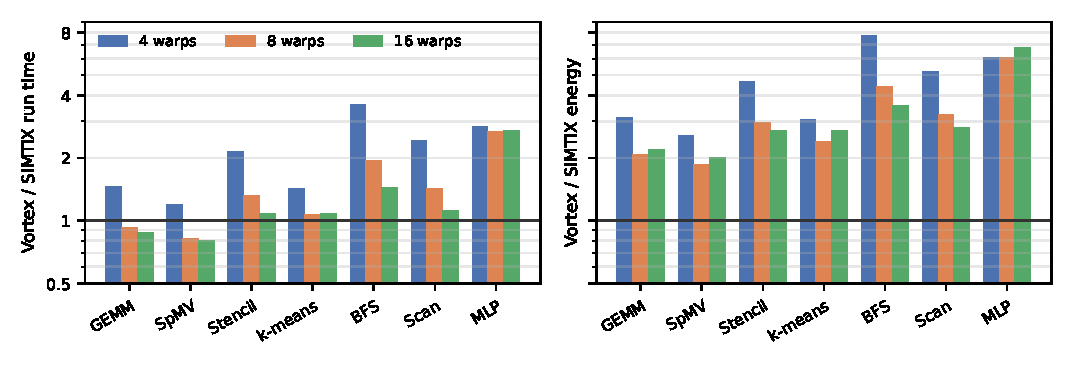
\includegraphics[width=\textwidth]{vortex_ratio.pdf}
\caption{Vortex run time (a) and energy (b) relative to SIMTiX for each
application and their geometric mean, with Vortex at 4, 8 and 16 warps of eight
threads. Run time uses each design's \Fmax; energy uses the vectorless power at
100~MHz. Bars above 1 favor SIMTiX, bars below 1 favor Vortex.}
\label{fig:vortex}
\end{figure*}

Table~\ref{tab:vortex} and Fig.~\ref{fig:vortex} compare the two designs. With
four warps each, Vortex takes $1.66$ to $4.99\times$ the cycles of SIMTiX. The
ratio has two factors. Vortex executes 1.08 to 2.20 times the warp instructions,
and 3.46 times for the MLP, which has no INT8 dot-product instruction on Vortex;
its kernels carry divergence and predicate instructions and compiled loop code
where SIMTiX runs hand-written assembly. Vortex also reaches a lower IPC, 0.25 to
0.43 against SIMTiX's 0.43 to 0.69, because four warps do not fill its longer
pipeline, while SIMTiX's two-stage pipeline needs only two runnable warps. With 16
warps Vortex's IPC rises to 0.47--0.66, exceeds SIMTiX's on SpMV, the stencil,
BFS and scan, and is within 4\% of it on GEMM, so most of its remaining cycle
deficit comes from its instruction count.

Vortex closes at 140.8~MHz, 39\% above SIMTiX's 101.6~MHz, and uses 5\% fewer
LUTs but 2.5 times the flip-flops, 2.9 times the block RAM and 55\% more power. In
run time, which includes the frequency difference, SIMTiX is $2.01\times$ faster
than four-warp Vortex in the geometric mean. Vortex at eight and 16 warps is
faster than SIMTiX on GEMM (0.92 and 0.88) and SpMV (0.82 and 0.80), whose regular
loops it executes with few extra instructions, while SIMTiX remains faster on BFS
($1.44\times$), scan ($1.12\times$) and the MLP ($2.71\times$) at 16 warps. Those
16 warps cost Vortex 30\% more LUTs than SIMTiX and 89\% more power. Per LUT,
SIMTiX delivers 1.46 to 1.90 times the performance of Vortex, and per watt three
to 4.3 times, at every Vortex warp count. The memory model matters little: Vortex's
cycles change by at most 9\% (the stencil) between its default
64-byte-per-cycle memory and the 128-bit bus with the IP latencies. SIMTiX's
frequency in this flow, 101.6~MHz, agrees with the board design's 101.0~MHz.

\subsection{Scaling With the Lane Count}\label{sec:evallanes}
\begin{figure}[t]
\centering
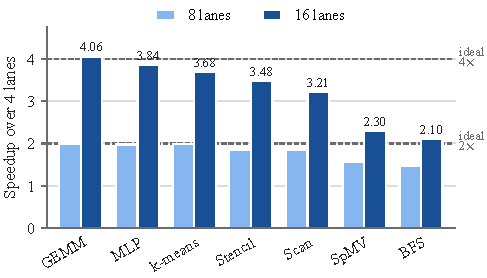
\includegraphics[width=\columnwidth]{lanes_speedup.pdf}
\caption{Speedup of each application at 8 and 16 lanes over a four-lane SIMTiX,
with four warps and a 16~KB L1 whose line is one word per lane. Dashed lines mark
linear speedup.}
\label{fig:lanes}
\end{figure}

The lane count $L$ is a parameter: it sets the warp width, the line of the memory
engine and the L1 (one word per lane, with the L1 kept at 16~KB) and the burst
length of the AXI4 master. Fig.~\ref{fig:lanes} shows the speedup over four lanes,
with four warps throughout; all seven applications pass their bit-exact checks at
every lane count. From eight to 16 lanes GEMM gains $2.03\times$, the MLP
$1.95\times$, the stencil $1.88\times$ and k-means $1.86\times$, while scan gains
$1.74\times$, SpMV $1.47\times$ and BFS $1.43\times$. GEMM, the stencil, k-means
and the MLP keep every lane active, and the scan 95\% of them. SpMV and BFS diverge
on their row and neighbor loops, where a warp runs until its longest row or
adjacency list ends, and their lane utilization falls from 66\% and 55\% at four
lanes to 59\% and 43\% at eight and 57\% and 34\% at 16. Their gathers also touch
about one line per lane, and the memory engine sends one request per line: from
eight to 16 lanes the warp instructions of SpMV halve, but its L1 accesses fall
only from 12,100 to 9,625, and its IPC drops from 0.43 to 0.33.

The cost grows faster than the lane count. Four lanes use 43,119 LUTs at
113.5~MHz and eight lanes 84,443 at 101.6~MHz. Placed, the 16-lane design
occupies 190,401 LUTs, 83\% of the device and 2.3 times the eight-lane design,
and 96\% of the device's configurable logic blocks hold some of its logic
\tbd{routed result}. Each lane's FPU stays at 4.8k LUTs, but the memory engine,
implemented alone in its board configuration, grows from 4,645 LUTs at four lanes
to 12,576 at eight and 42,474 at 16, by 2.7 and then 3.4 times per doubling; all
three meet 100~MHz. The engine selects the word of every lane from a line that
itself holds one word per lane, places every lane's store data into that line,
and, for the aggregated AMOs, compares the word addresses of every pair of lanes.
These structures grow with the square of the lane count. Wider warps are
therefore limited by the memory engine rather than by the lanes, and beyond eight
lanes more cores, or an engine that serves part of a warp per cycle, are the
better way to add throughput.

The 16-lane run also exposed the stack bound of Section~\ref{sec:arch}. Our stack
had eight frames, which by the bound suffices for eight lanes. In SpMV at 16
lanes, a warp whose rows have more than eight different lengths leaves its loop at
more than eight different iterations, pushing a frame each time, and overflowed
the stack. Sizing the stack by the lane count removed the failure; at eight lanes
the design is unchanged.

\subsection{Measurements on the Board}\label{sec:evalboard}
\begin{table}[t]
\caption{Applications on the ZCU104: SIMTiX at 100~MHz Against One Cortex-A53
Core at 1.2~GHz}
\label{tab:board}
\centering\footnotesize
\setlength{\tabcolsep}{3pt}
\begin{tabular}{lrrrrrr}
\toprule
App. & A53 & SIMTiX & Speedup & \multicolumn{2}{c}{Power above idle (W)} & Energy\\
\cmidrule(lr){5-6}
 & (ms) & (ms) & & A53 & SIMTiX & ratio\\
\midrule
GEMM    & \tbd{} & \tbd{} & \tbd{} & \tbd{} & \tbd{} & \tbd{}\\
SpMV    & \tbd{} & \tbd{} & \tbd{} & \tbd{} & \tbd{} & \tbd{}\\
Stencil & \tbd{} & \tbd{} & \tbd{} & \tbd{} & \tbd{} & \tbd{}\\
k-means & \tbd{} & \tbd{} & \tbd{} & \tbd{} & \tbd{} & \tbd{}\\
BFS     & \tbd{} & \tbd{} & \tbd{} & \tbd{} & \tbd{} & \tbd{}\\
Scan    & \tbd{} & \tbd{} & \tbd{} & \tbd{} & \tbd{} & \tbd{}\\
MLP     & \tbd{} & \tbd{} & \tbd{} & \tbd{} & \tbd{} & \tbd{}\\
\bottomrule
\end{tabular}

\vspace{2pt}
\begin{minipage}{\columnwidth}\footnotesize
Inputs: the board inputs of Table~\ref{tab:apps}. Power: 12~V board input,
averaged over 2~s of repetitions. Energy ratio: A53 energy over SIMTiX energy,
each the run time times the power above idle.
\end{minipage}
\end{table}

The host program runs every application on the DRAM-sized input of
Table~\ref{tab:apps}, first on the accelerator and then on one A53 core with an
ordinary sequential algorithm in C compiled at \texttt{-O2}: a queue for BFS, a
running sum for the scan and the $i$-$k$-$j$ loop order for GEMM. The FP32
references perform the kernels' operations in the same order, so every output of
the accelerator is compared exactly with the A53's. Times come from the A53's
global timer; the accelerator time runs from the first GO to the last DONE and
includes the host's work between launches. For power, each phase (idle,
accelerator, A53) is repeated for 2~s, and between repetitions, at most every
50~ms, the host reads the board's monitors over I$^2$C: an INA226 on the 12~V
input and the output rails of two IRPS5401 regulators. \tbd{Results: speedups,
power above idle, energy; which rails the accelerator's power appears on.}

%==============================================================================
\section{Limitations}\label{sec:disc}
%==============================================================================
SIMTiX trades frequency for IPC. Its two-stage pipeline reads the LUTRAM RFs and
decodes in the issue cycle, and its critical paths are the stage-0 addition of the
FPU and the issue logic; Vortex's deeper pipeline closes at a 39\% higher
frequency but needs more warps to fill. The power in the Vortex comparison is a
vectorless estimate for both designs; the board measurements cover SIMTiX and the
A53 only. SIMTiX has no compiler: its kernels are hand-written assembly, while
Vortex's are compiled by LLVM, so part of Vortex's 1.72 times instruction count
reflects compiled code rather than the instruction set; the IPC comparison
divides this effect out. Both designs were evaluated as single cores;
multi-core configurations, which Vortex supports with an L2 cache and an OpenCL
stack, were not. The AMOs exclude load-reserved and store-conditional.

%==============================================================================
\section{Conclusion}
%==============================================================================
This paper describes the architecture and implementation of SIMTiX, a SIMT
accelerator of eight lanes and four warps for FPGA systems-on-chip. It includes a
non-blocking L1, a multi-context memory engine, AXI4 access to DDR4, shuffles,
barriers, atomics and FP32/FP16 arithmetic in 81k LUTs of a mid-size device, and
the complete board design closes timing at 101.0~MHz. Line-aggregated AMOs serve
all lanes of an atomic that share a line with one read and one write while
preserving the results of serial execution, which reduces the memory requests of
a histogram by $3.4\times$ for 2,551 LUTs. On the same device and flow as Vortex
with the same geometry, SIMTiX runs seven applications in $2.01\times$ less time
and with $4.3\times$ less estimated energy; Vortex closes at a higher frequency and
overtakes SIMTiX on regular kernels only with 16 warps and 30\% more LUTs. Beyond
eight lanes the memory engine grows almost with the square of the lane count, so
wider SIMT engines on FPGAs should add cores or serve part of a warp per cycle
rather than widen the warp. \tbd{one sentence with the board result.}

%==============================================================================
\section*{Acknowledgment}
%==============================================================================
The authors used a large language model (Anthropic Claude) to assist with build
and analysis scripting and with editing this manuscript. The design, the
experiments and their interpretation are the authors' own, and the authors checked
every reported result.

%==============================================================================
\begin{thebibliography}{99}
\bibitem{tesla} E.~Lindholm, J.~Nickolls, S.~Oberman, and J.~Montrym,
``NVIDIA Tesla: A unified graphics and computing architecture,''
\emph{IEEE Micro}, vol.~28, no.~2, pp.~39--55, Mar. 2008.
\bibitem{aamodt} T.~M.~Aamodt, W.~W.~L.~Fung, and T.~G.~Rogers,
\emph{General-Purpose Graphics Processor Architectures}. San Rafael, CA, USA:
Morgan \& Claypool, 2018.
\bibitem{vortex} B.~Tine, K.~P.~Yalamarthy, F.~Elsabbagh, and H.~Kim,
``Vortex: Extending the RISC-V ISA for GPGPU and 3D-graphics,'' in
\emph{Proc. IEEE/ACM Int. Symp. Microarchitecture (MICRO)}, 2021, pp.~754--766.
\bibitem{ventus25} J.~Li \emph{et al.}, ``RISC-V-based GPGPU with vector
capabilities for high-performance computing,'' \emph{IEEE Trans. Very Large Scale
Integr. (VLSI) Syst.}, vol.~33, no.~8, pp.~2239--2252, Aug. 2025.
\bibitem{egpu} M.~Langhammer and G.~A.~Constantinides, ``eGPU: A 750 MHz class
soft GPGPU for FPGA,'' in \emph{Proc. Int. Conf. Field-Programmable Logic Appl.
(FPL)}, 2023.
\bibitem{flexgrip} K.~Andryc, M.~Merchant, and R.~Tessier, ``FlexGrip: A soft
GPGPU for FPGAs,'' in \emph{Proc. Int. Conf. Field-Programmable Technol. (FPT)},
2013.
\bibitem{fgpu} M.~Al~Kadi, B.~Janssen, and M.~H\"ubner, ``FGPU: An
SIMT-architecture for FPGAs,'' in \emph{Proc. ACM/SIGDA Int. Symp.
Field-Programmable Gate Arrays (FPGA)}, 2016, pp.~254--263.
\bibitem{miaow} R.~Balasubramanian \emph{et al.}, ``Enabling GPGPU low-level
hardware explorations with MIAOW: An open-source RTL implementation of a GPGPU,''
\emph{ACM Trans. Archit. Code Optim.}, vol.~12, no.~2, 2015.
\bibitem{nyuzi} J.~Bush, P.~Dexter, T.~N.~Miller, and A.~Carpenter, ``Nyami: A
synthesizable GPU architectural model for general-purpose and graphics-specific
workloads,'' in \emph{Proc. IEEE Int. Symp. Perform. Anal. Syst. Softw.
(ISPASS)}, 2015.
\bibitem{simty} S.~Collange, ``Simty: Generalized SIMT execution on RISC-V,'' in
\emph{Proc. Workshop Comput. Archit. Res. RISC-V (CARRV)}, 2017.
\bibitem{fung} W.~W.~L.~Fung, I.~Sham, G.~Yuan, and T.~M.~Aamodt, ``Dynamic warp
formation and scheduling for efficient GPU control flow,'' in \emph{Proc. IEEE/ACM
Int. Symp. Microarchitecture (MICRO)}, 2007, pp.~407--420.
\bibitem{fermi} NVIDIA, ``NVIDIA's next generation CUDA compute architecture:
Fermi,'' White Paper, 2009.
\bibitem{dab} Y.~H.~Chou, C.~Ng, S.~Cattell, J.~Intan, M.~D.~Sinclair,
J.~Devietti, T.~G.~Rogers, and T.~M.~Aamodt, ``Deterministic atomic buffering,''
in \emph{Proc. IEEE/ACM Int. Symp. Microarchitecture (MICRO)}, 2020,
pp.~981--995.
\bibitem{franey} S.~Franey and M.~Lipasti, ``Accelerating atomic operations on
GPGPUs,'' in \emph{Proc. IEEE/ACM Int. Symp. Networks-on-Chip (NOCS)}, 2013,
pp.~1--8.
\bibitem{phi} A.~Mukkara, N.~Beckmann, and D.~Sanchez, ``PHI: Architectural
support for synchronization- and bandwidth-efficient commutative scatter
updates,'' in \emph{Proc. IEEE/ACM Int. Symp. Microarchitecture (MICRO)}, 2019,
pp.~1009--1022.
\bibitem{warpagg} A.~Adinets, ``CUDA pro tip: Optimized filtering with
warp-aggregated atomics,'' NVIDIA Developer Blog, Oct. 2014.
\bibitem{figueroa} S.~A.~Figueroa, ``When is double rounding innocuous?''
\emph{ACM SIGNUM Newsl.}, vol.~30, no.~3, pp.~21--26, 1995.
\bibitem{ieee754} \emph{IEEE Standard for Floating-Point Arithmetic}, IEEE Std
754-2019, 2019.
\end{thebibliography}

\end{document}
